% Auto-generated by the analysis pipeline — do not edit
% \input this inside a figure environment.
% Requires the subcaption and graphicx packages.
% Each panel carries its own % ADD THEORY CURVE BELOW marker.
\begin{subfigure}[t]{0.485\textwidth}
\centering
\resizebox{\linewidth}{!}{
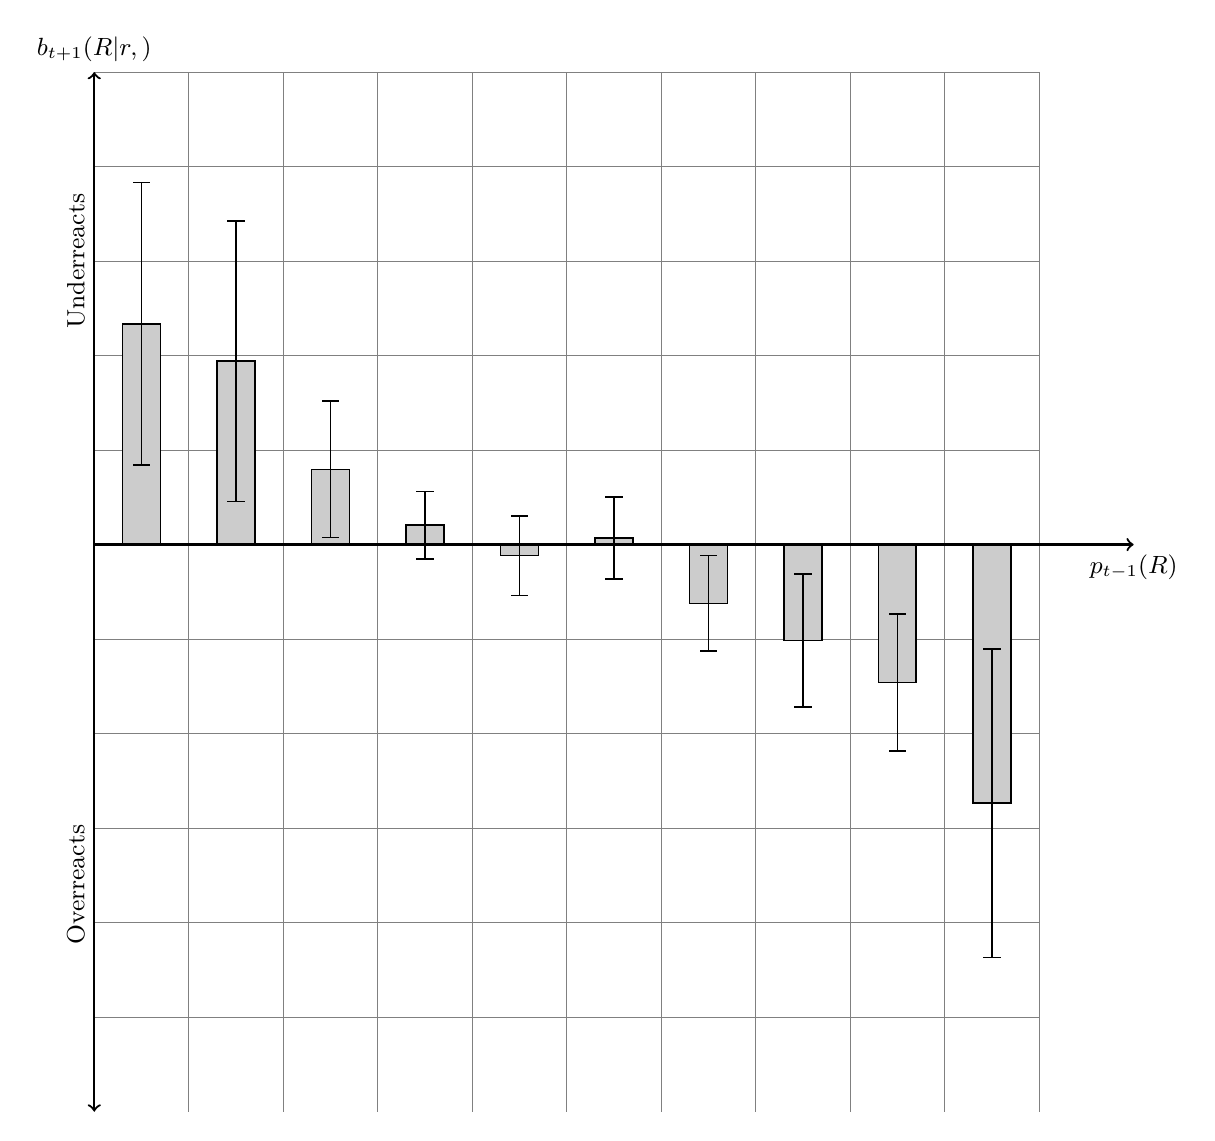
\begin{tikzpicture}[scale=12]
\draw[help lines,step=0.1] (0,-0.6) grid (1,0.5);
\filldraw[opaque,white!80!black] (0.03,0) rectangle (0.07,0.2337);
\draw[line width=0.6] (0.03,0) rectangle (0.07,0.2337);
\draw[line width=0.6,|-|] (0.05,0.0835) -- (0.05,0.3839);
\filldraw[opaque,white!80!black] (0.13,0) rectangle (0.17,0.1941);
\draw[line width=0.6] (0.13,0) rectangle (0.17,0.1941);
\draw[line width=0.6,|-|] (0.15,0.0446) -- (0.15,0.3436);
\filldraw[opaque,white!80!black] (0.23,0) rectangle (0.27,0.0796);
\draw[line width=0.6] (0.23,0) rectangle (0.27,0.0796);
\draw[line width=0.6,|-|] (0.25,0.0067) -- (0.25,0.1525);
\filldraw[opaque,white!80!black] (0.33,0) rectangle (0.37,0.0205);
\draw[line width=0.6] (0.33,0) rectangle (0.37,0.0205);
\draw[line width=0.6,|-|] (0.35,-0.0162) -- (0.35,0.0571);
\filldraw[opaque,white!80!black] (0.43,0) rectangle (0.47,-0.0117);
\draw[line width=0.6] (0.43,0) rectangle (0.47,-0.0117);
\draw[line width=0.6,|-|] (0.45,-0.0547) -- (0.45,0.0313);
\filldraw[opaque,white!80!black] (0.53,0) rectangle (0.57,0.0071);
\draw[line width=0.6] (0.53,0) rectangle (0.57,0.0071);
\draw[line width=0.6,|-|] (0.55,-0.0372) -- (0.55,0.0515);
\filldraw[opaque,white!80!black] (0.63,0) rectangle (0.67,-0.0622);
\draw[line width=0.6] (0.63,0) rectangle (0.67,-0.0622);
\draw[line width=0.6,|-|] (0.65,-0.1138) -- (0.65,-0.0106);
\filldraw[opaque,white!80!black] (0.73,0) rectangle (0.77,-0.1016);
\draw[line width=0.6] (0.73,0) rectangle (0.77,-0.1016);
\draw[line width=0.6,|-|] (0.75,-0.1728) -- (0.75,-0.0305);
\filldraw[opaque,white!80!black] (0.83,0) rectangle (0.87,-0.1458);
\draw[line width=0.6] (0.83,0) rectangle (0.87,-0.1458);
\draw[line width=0.6,|-|] (0.85,-0.2190) -- (0.85,-0.0727);
\filldraw[opaque,white!80!black] (0.93,0) rectangle (0.97,-0.2738);
\draw[line width=0.6] (0.93,0) rectangle (0.97,-0.2738);
\draw[line width=0.6,|-|] (0.95,-0.4379) -- (0.95,-0.1098);
\draw[line width=0.8,->]  (0,0) -- (1.1,0) node[below] {\small{$p_{t-1}(R)$}};
\draw[line width=0.8,<->] (0,-0.6) -- (0,0.5) node[above] {\small{$b_{t+1}(R|r,\xmark)$}};
\draw (0,0.30) node[above,rotate=90] {\small{Underreacts}};
\draw (0,-0.36) node[above,rotate=90] {\small{Overreacts}};
% ADD THEORY CURVE BELOW
\end{tikzpicture}
}
\subcaption{$(H_{0,0})$: 0 retractions / 0 confirmations}
\end{subfigure}
\hfill
\begin{subfigure}[t]{0.485\textwidth}
\centering
\resizebox{\linewidth}{!}{
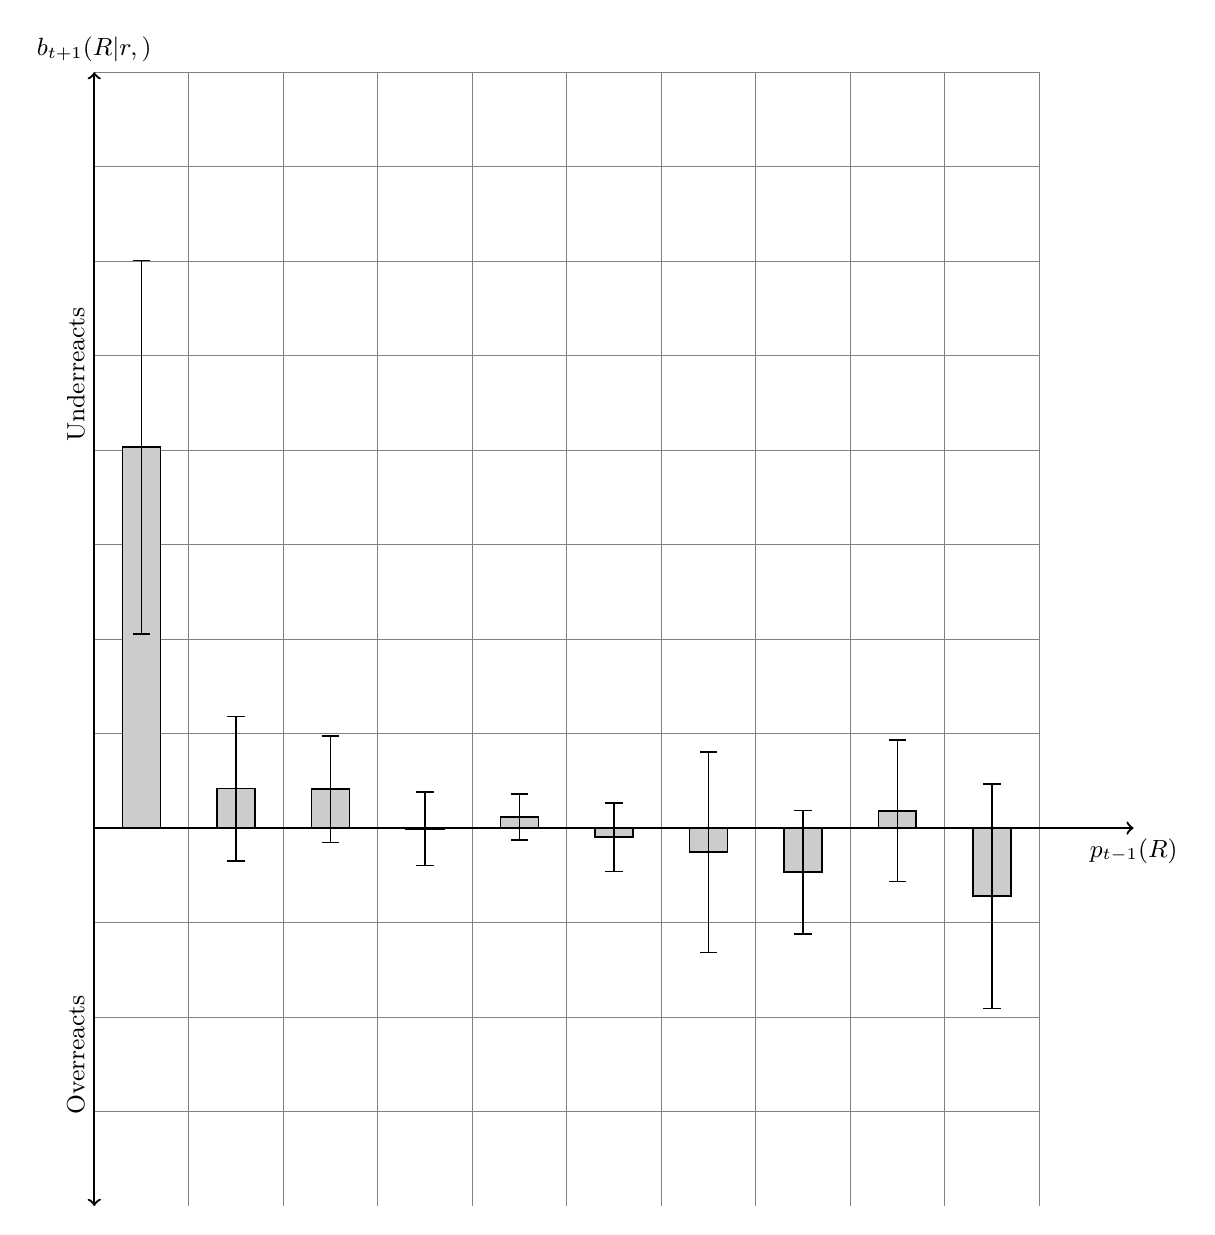
\begin{tikzpicture}[scale=12]
\draw[help lines,step=0.1] (0,-0.4) grid (1,0.8);
\filldraw[opaque,white!80!black] (0.03,0) rectangle (0.07,0.4031);
\draw[line width=0.6] (0.03,0) rectangle (0.07,0.4031);
\draw[line width=0.6,|-|] (0.05,0.2047) -- (0.05,0.6015);
\filldraw[opaque,white!80!black] (0.13,0) rectangle (0.17,0.0417);
\draw[line width=0.6] (0.13,0) rectangle (0.17,0.0417);
\draw[line width=0.6,|-|] (0.15,-0.0355) -- (0.15,0.1188);
\filldraw[opaque,white!80!black] (0.23,0) rectangle (0.27,0.0412);
\draw[line width=0.6] (0.23,0) rectangle (0.27,0.0412);
\draw[line width=0.6,|-|] (0.25,-0.0163) -- (0.25,0.0986);
\filldraw[opaque,white!80!black] (0.33,0) rectangle (0.37,-0.0008);
\draw[line width=0.6] (0.33,0) rectangle (0.37,-0.0008);
\draw[line width=0.6,|-|] (0.35,-0.0405) -- (0.35,0.0388);
\filldraw[opaque,white!80!black] (0.43,0) rectangle (0.47,0.0117);
\draw[line width=0.6] (0.43,0) rectangle (0.47,0.0117);
\draw[line width=0.6,|-|] (0.45,-0.0134) -- (0.45,0.0369);
\filldraw[opaque,white!80!black] (0.53,0) rectangle (0.57,-0.0097);
\draw[line width=0.6] (0.53,0) rectangle (0.57,-0.0097);
\draw[line width=0.6,|-|] (0.55,-0.0468) -- (0.55,0.0275);
\filldraw[opaque,white!80!black] (0.63,0) rectangle (0.67,-0.0255);
\draw[line width=0.6] (0.63,0) rectangle (0.67,-0.0255);
\draw[line width=0.6,|-|] (0.65,-0.1325) -- (0.65,0.0816);
\filldraw[opaque,white!80!black] (0.73,0) rectangle (0.77,-0.0468);
\draw[line width=0.6] (0.73,0) rectangle (0.77,-0.0468);
\draw[line width=0.6,|-|] (0.75,-0.1133) -- (0.75,0.0196);
\filldraw[opaque,white!80!black] (0.83,0) rectangle (0.87,0.0183);
\draw[line width=0.6] (0.83,0) rectangle (0.87,0.0183);
\draw[line width=0.6,|-|] (0.85,-0.0576) -- (0.85,0.0943);
\filldraw[opaque,white!80!black] (0.93,0) rectangle (0.97,-0.0722);
\draw[line width=0.6] (0.93,0) rectangle (0.97,-0.0722);
\draw[line width=0.6,|-|] (0.95,-0.1918) -- (0.95,0.0473);
\draw[line width=0.8,->]  (0,0) -- (1.1,0) node[below] {\small{$p_{t-1}(R)$}};
\draw[line width=0.8,<->] (0,-0.4) -- (0,0.8) node[above] {\small{$b_{t+1}(R|r,\xmark)$}};
\draw (0,0.48) node[above,rotate=90] {\small{Underreacts}};
\draw (0,-0.24) node[above,rotate=90] {\small{Overreacts}};
% ADD THEORY CURVE BELOW
\end{tikzpicture}
}
\subcaption{$(H_{1,0})$: 1 retraction / 0 confirmations}
\end{subfigure}
\\[1.5ex]
\begin{subfigure}[t]{0.485\textwidth}
\centering
\resizebox{\linewidth}{!}{
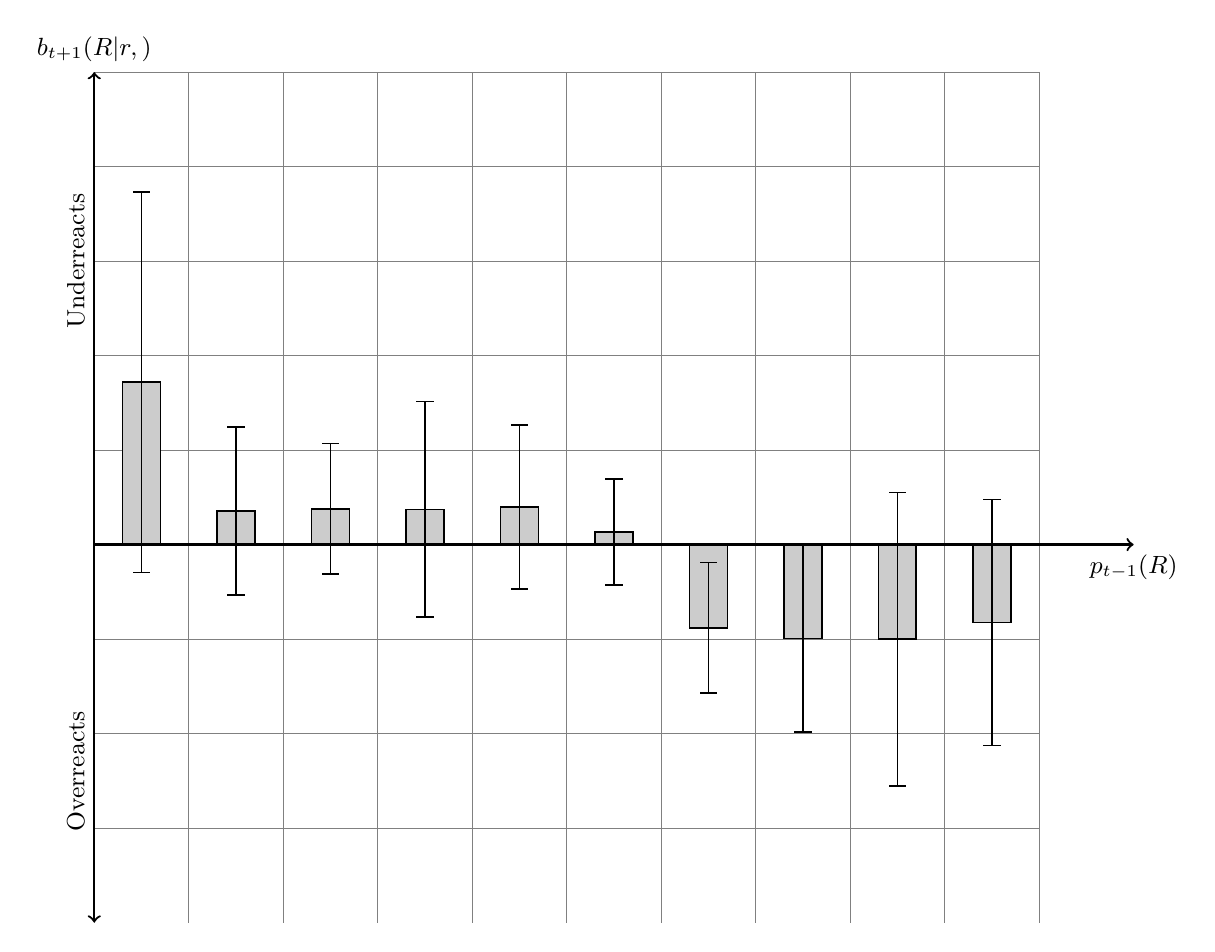
\begin{tikzpicture}[scale=12]
\draw[help lines,step=0.1] (0,-0.4) grid (1,0.5);
\filldraw[opaque,white!80!black] (0.03,0) rectangle (0.07,0.1718);
\draw[line width=0.6] (0.03,0) rectangle (0.07,0.1718);
\draw[line width=0.6,|-|] (0.05,-0.0306) -- (0.05,0.3742);
\filldraw[opaque,white!80!black] (0.13,0) rectangle (0.17,0.0356);
\draw[line width=0.6] (0.13,0) rectangle (0.17,0.0356);
\draw[line width=0.6,|-|] (0.15,-0.0540) -- (0.15,0.1251);
\filldraw[opaque,white!80!black] (0.23,0) rectangle (0.27,0.0378);
\draw[line width=0.6] (0.23,0) rectangle (0.27,0.0378);
\draw[line width=0.6,|-|] (0.25,-0.0323) -- (0.25,0.1079);
\filldraw[opaque,white!80!black] (0.33,0) rectangle (0.37,0.0373);
\draw[line width=0.6] (0.33,0) rectangle (0.37,0.0373);
\draw[line width=0.6,|-|] (0.35,-0.0777) -- (0.35,0.1523);
\filldraw[opaque,white!80!black] (0.43,0) rectangle (0.47,0.0395);
\draw[line width=0.6] (0.43,0) rectangle (0.47,0.0395);
\draw[line width=0.6,|-|] (0.45,-0.0482) -- (0.45,0.1272);
\filldraw[opaque,white!80!black] (0.53,0) rectangle (0.57,0.0133);
\draw[line width=0.6] (0.53,0) rectangle (0.57,0.0133);
\draw[line width=0.6,|-|] (0.55,-0.0438) -- (0.55,0.0705);
\filldraw[opaque,white!80!black] (0.63,0) rectangle (0.67,-0.0880);
\draw[line width=0.6] (0.63,0) rectangle (0.67,-0.0880);
\draw[line width=0.6,|-|] (0.65,-0.1580) -- (0.65,-0.0180);
\filldraw[opaque,white!80!black] (0.73,0) rectangle (0.77,-0.0994);
\draw[line width=0.6] (0.73,0) rectangle (0.77,-0.0994);
\draw[line width=0.6,|-|] (0.75,-0.1991) -- (0.75,0.0004);
\filldraw[opaque,white!80!black] (0.83,0) rectangle (0.87,-0.1000);
\draw[line width=0.6] (0.83,0) rectangle (0.87,-0.1000);
\draw[line width=0.6,|-|] (0.85,-0.2561) -- (0.85,0.0561);
\filldraw[opaque,white!80!black] (0.93,0) rectangle (0.97,-0.0825);
\draw[line width=0.6] (0.93,0) rectangle (0.97,-0.0825);
\draw[line width=0.6,|-|] (0.95,-0.2135) -- (0.95,0.0485);
\draw[line width=0.8,->]  (0,0) -- (1.1,0) node[below] {\small{$p_{t-1}(R)$}};
\draw[line width=0.8,<->] (0,-0.4) -- (0,0.5) node[above] {\small{$b_{t+1}(R|r,\xmark)$}};
\draw (0,0.30) node[above,rotate=90] {\small{Underreacts}};
\draw (0,-0.24) node[above,rotate=90] {\small{Overreacts}};
% ADD THEORY CURVE BELOW
\end{tikzpicture}
}
\subcaption{$(H_{0,1})$: 0 retractions / 1 confirmation}
\end{subfigure}
\hfill
\begin{subfigure}[t]{0.485\textwidth}
\centering
\resizebox{\linewidth}{!}{
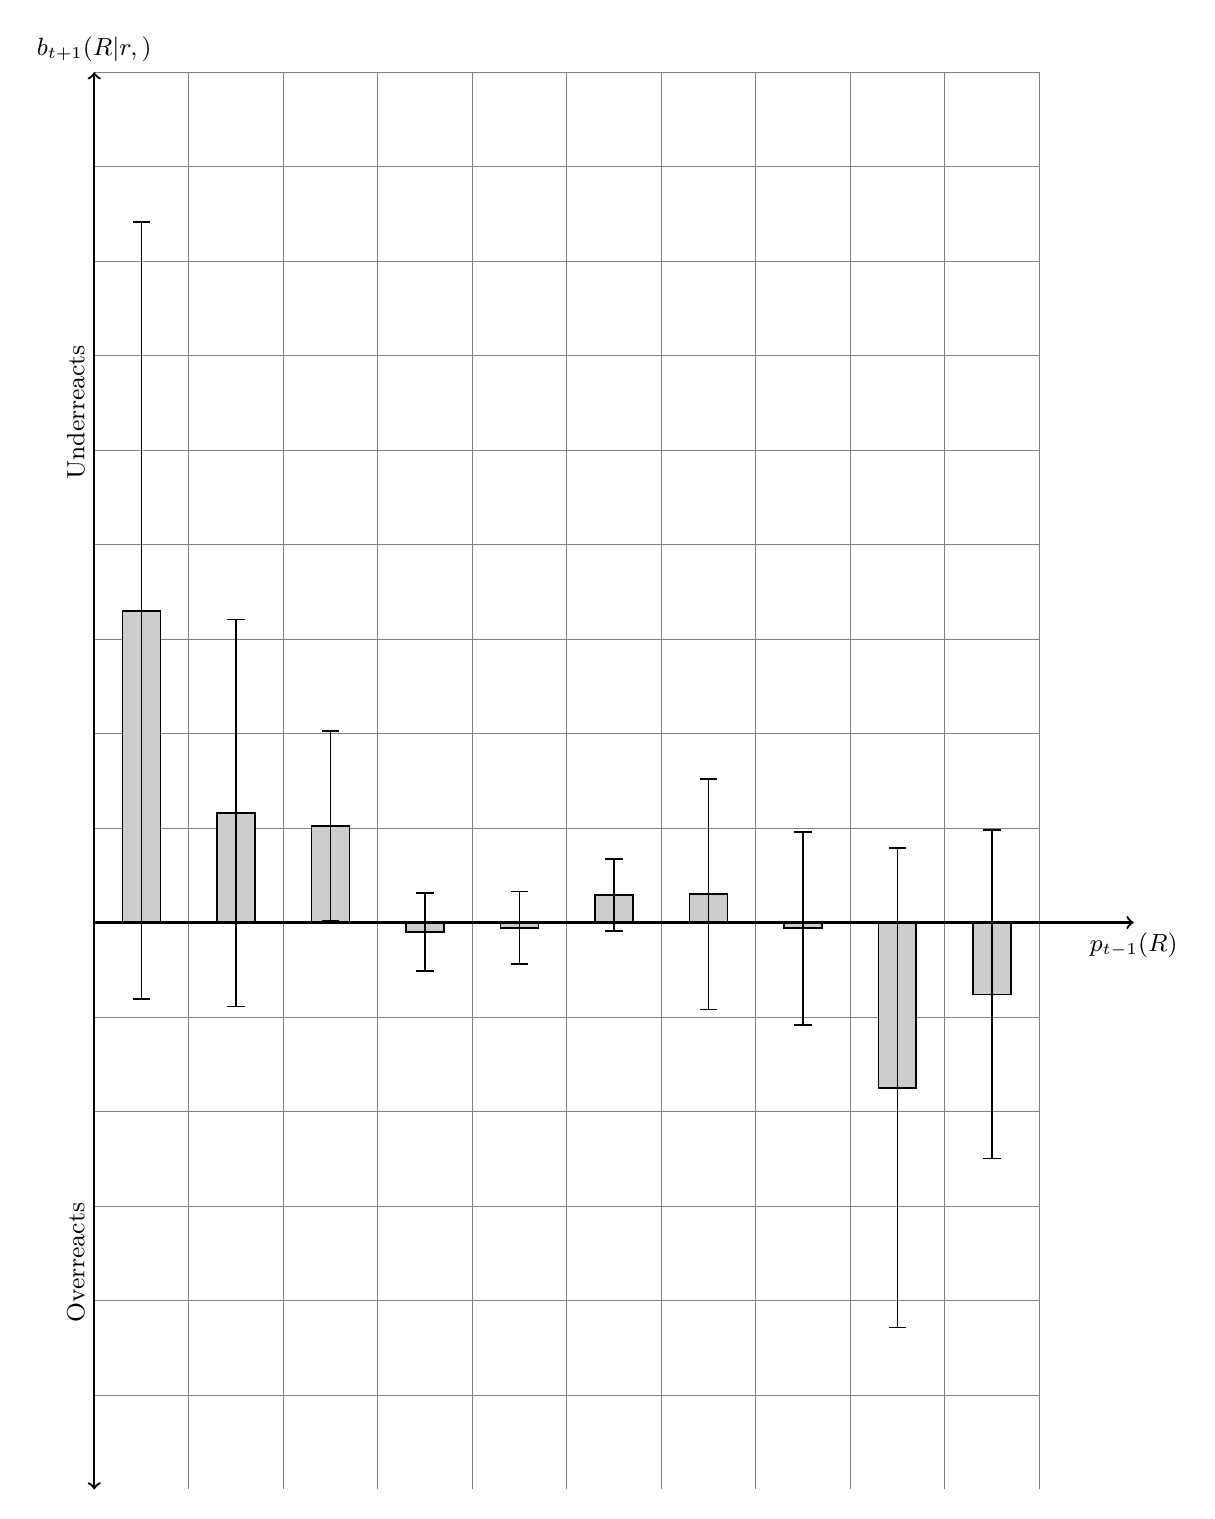
\begin{tikzpicture}[scale=12]
\draw[help lines,step=0.1] (0,-0.6) grid (1,0.9);
\filldraw[opaque,white!80!black] (0.03,0) rectangle (0.07,0.3300);
\draw[line width=0.6] (0.03,0) rectangle (0.07,0.3300);
\draw[line width=0.6,|-|] (0.05,-0.0821) -- (0.05,0.7421);
\filldraw[opaque,white!80!black] (0.13,0) rectangle (0.17,0.1160);
\draw[line width=0.6] (0.13,0) rectangle (0.17,0.1160);
\draw[line width=0.6,|-|] (0.15,-0.0896) -- (0.15,0.3216);
\filldraw[opaque,white!80!black] (0.23,0) rectangle (0.27,0.1025);
\draw[line width=0.6] (0.23,0) rectangle (0.27,0.1025);
\draw[line width=0.6,|-|] (0.25,0.0014) -- (0.25,0.2036);
\filldraw[opaque,white!80!black] (0.33,0) rectangle (0.37,-0.0100);
\draw[line width=0.6] (0.33,0) rectangle (0.37,-0.0100);
\draw[line width=0.6,|-|] (0.35,-0.0519) -- (0.35,0.0319);
\filldraw[opaque,white!80!black] (0.43,0) rectangle (0.47,-0.0056);
\draw[line width=0.6] (0.43,0) rectangle (0.47,-0.0056);
\draw[line width=0.6,|-|] (0.45,-0.0449) -- (0.45,0.0336);
\filldraw[opaque,white!80!black] (0.53,0) rectangle (0.57,0.0291);
\draw[line width=0.6] (0.53,0) rectangle (0.57,0.0291);
\draw[line width=0.6,|-|] (0.55,-0.0102) -- (0.55,0.0684);
\filldraw[opaque,white!80!black] (0.63,0) rectangle (0.67,0.0300);
\draw[line width=0.6] (0.63,0) rectangle (0.67,0.0300);
\draw[line width=0.6,|-|] (0.65,-0.0928) -- (0.65,0.1528);
\filldraw[opaque,white!80!black] (0.73,0) rectangle (0.77,-0.0060);
\draw[line width=0.6] (0.73,0) rectangle (0.77,-0.0060);
\draw[line width=0.6,|-|] (0.75,-0.1090) -- (0.75,0.0970);
\filldraw[opaque,white!80!black] (0.83,0) rectangle (0.87,-0.1750);
\draw[line width=0.6] (0.83,0) rectangle (0.87,-0.1750);
\draw[line width=0.6,|-|] (0.85,-0.4296) -- (0.85,0.0796);
\filldraw[opaque,white!80!black] (0.93,0) rectangle (0.97,-0.0760);
\draw[line width=0.6] (0.93,0) rectangle (0.97,-0.0760);
\draw[line width=0.6,|-|] (0.95,-0.2505) -- (0.95,0.0985);
\draw[line width=0.8,->]  (0,0) -- (1.1,0) node[below] {\small{$p_{t-1}(R)$}};
\draw[line width=0.8,<->] (0,-0.6) -- (0,0.9) node[above] {\small{$b_{t+1}(R|r,\xmark)$}};
\draw (0,0.54) node[above,rotate=90] {\small{Underreacts}};
\draw (0,-0.36) node[above,rotate=90] {\small{Overreacts}};
% ADD THEORY CURVE BELOW
\end{tikzpicture}
}
\subcaption{$(H_{2,0})$: 2 retractions / 0 confirmations}
\end{subfigure}
\\[1.5ex]
\begin{subfigure}[t]{0.485\textwidth}
\centering
\resizebox{\linewidth}{!}{
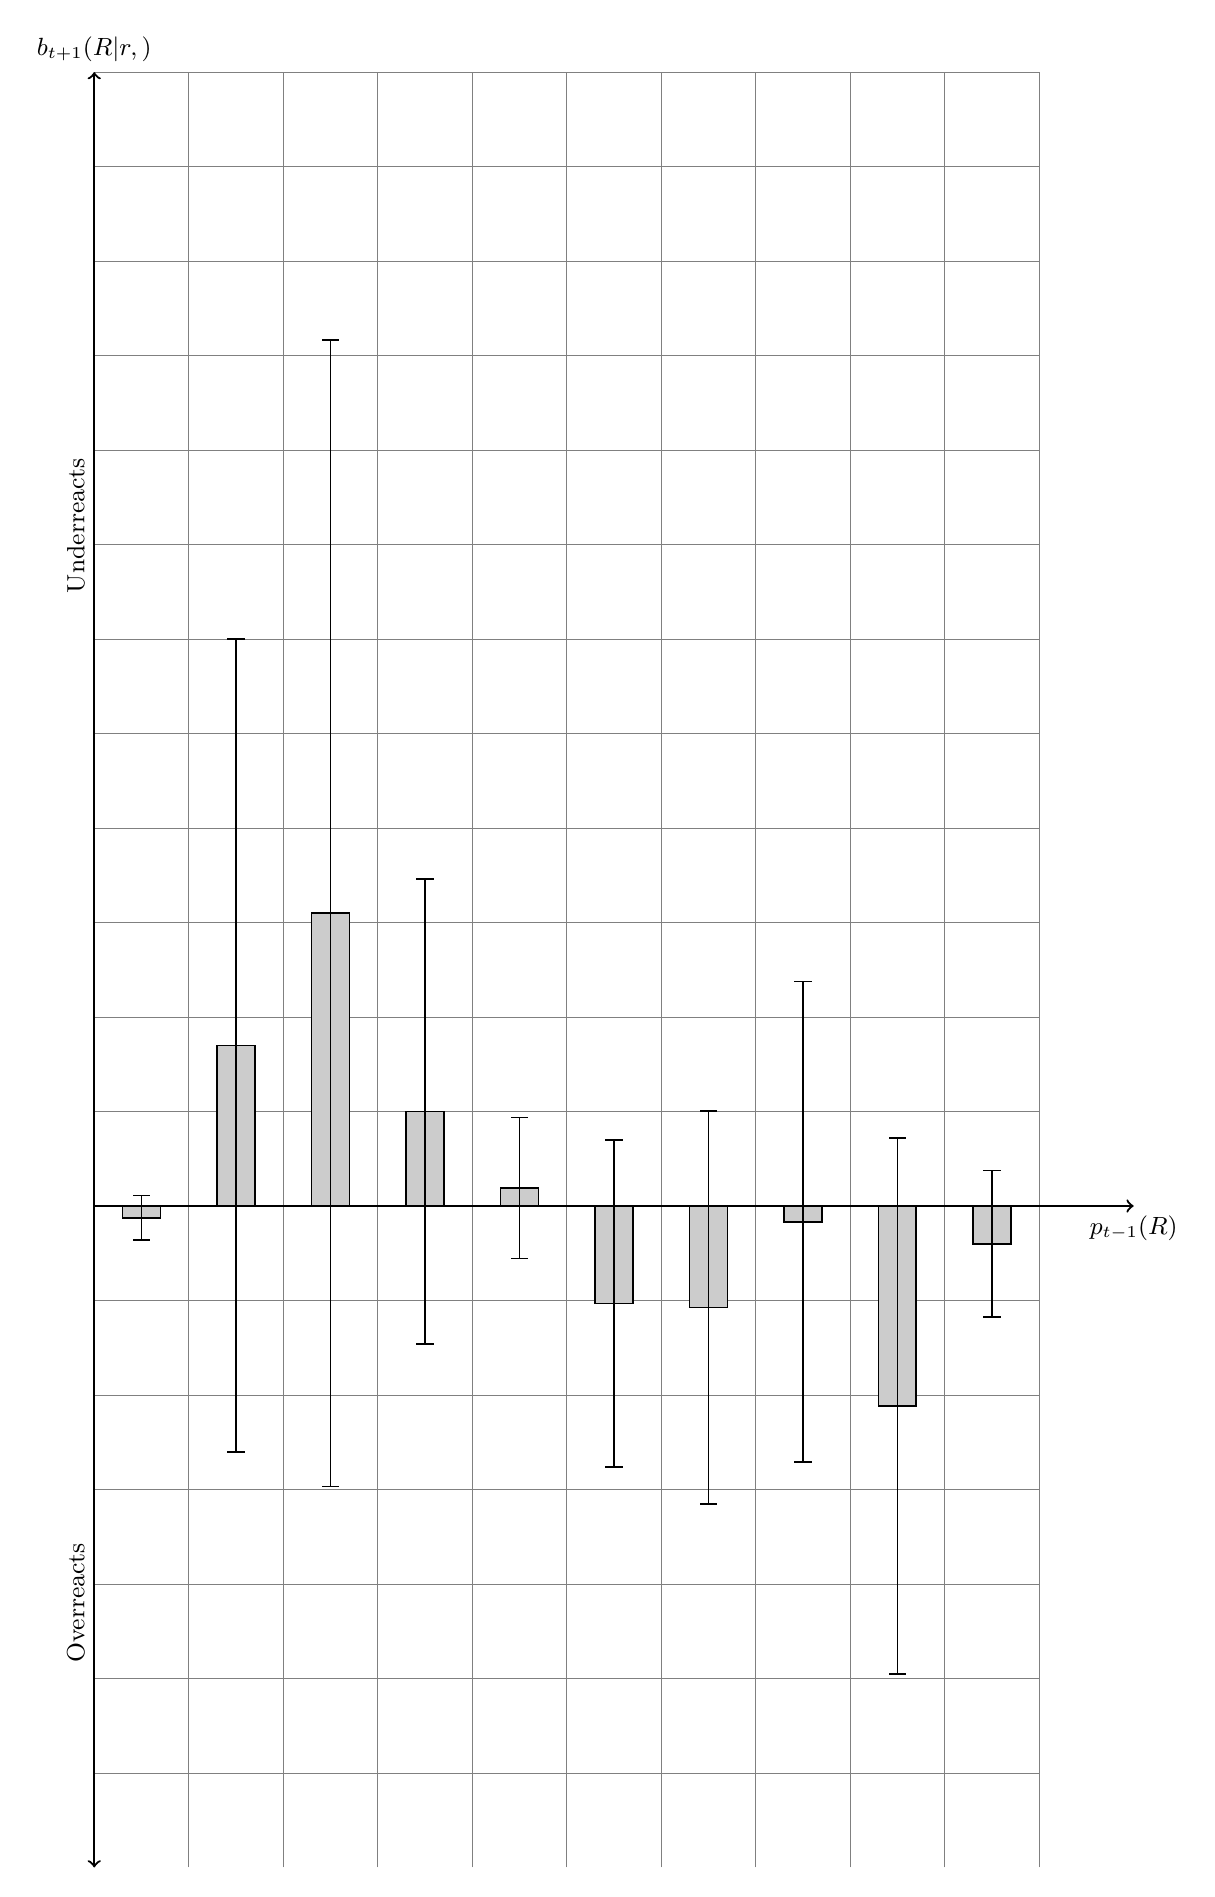
\begin{tikzpicture}[scale=12]
\draw[help lines,step=0.1] (0,-0.7) grid (1,1.2);
\filldraw[opaque,white!80!black] (0.03,0) rectangle (0.07,-0.0125);
\draw[line width=0.6] (0.03,0) rectangle (0.07,-0.0125);
\draw[line width=0.6,|-|] (0.05,-0.0370) -- (0.05,0.0120);
\filldraw[opaque,white!80!black] (0.13,0) rectangle (0.17,0.1700);
\draw[line width=0.6] (0.13,0) rectangle (0.17,0.1700);
\draw[line width=0.6,|-|] (0.15,-0.2612) -- (0.15,0.6012);
\filldraw[opaque,white!80!black] (0.23,0) rectangle (0.27,0.3100);
\draw[line width=0.6] (0.23,0) rectangle (0.27,0.3100);
\draw[line width=0.6,|-|] (0.25,-0.2976) -- (0.25,0.9176);
\filldraw[opaque,white!80!black] (0.33,0) rectangle (0.37,0.1000);
\draw[line width=0.6] (0.33,0) rectangle (0.37,0.1000);
\draw[line width=0.6,|-|] (0.35,-0.1466) -- (0.35,0.3466);
\filldraw[opaque,white!80!black] (0.43,0) rectangle (0.47,0.0190);
\draw[line width=0.6] (0.43,0) rectangle (0.47,0.0190);
\draw[line width=0.6,|-|] (0.45,-0.0566) -- (0.45,0.0946);
\filldraw[opaque,white!80!black] (0.53,0) rectangle (0.57,-0.1033);
\draw[line width=0.6] (0.53,0) rectangle (0.57,-0.1033);
\draw[line width=0.6,|-|] (0.55,-0.2773) -- (0.55,0.0706);
\filldraw[opaque,white!80!black] (0.63,0) rectangle (0.67,-0.1075);
\draw[line width=0.6] (0.63,0) rectangle (0.67,-0.1075);
\draw[line width=0.6,|-|] (0.65,-0.3164) -- (0.65,0.1014);
\filldraw[opaque,white!80!black] (0.73,0) rectangle (0.77,-0.0167);
\draw[line width=0.6] (0.73,0) rectangle (0.77,-0.0167);
\draw[line width=0.6,|-|] (0.75,-0.2718) -- (0.75,0.2385);
\filldraw[opaque,white!80!black] (0.83,0) rectangle (0.87,-0.2117);
\draw[line width=0.6] (0.83,0) rectangle (0.87,-0.2117);
\draw[line width=0.6,|-|] (0.85,-0.4961) -- (0.85,0.0727);
\filldraw[opaque,white!80!black] (0.93,0) rectangle (0.97,-0.0400);
\draw[line width=0.6] (0.93,0) rectangle (0.97,-0.0400);
\draw[line width=0.6,|-|] (0.95,-0.1184) -- (0.95,0.0384);
\draw[line width=0.8,->]  (0,0) -- (1.1,0) node[below] {\small{$p_{t-1}(R)$}};
\draw[line width=0.8,<->] (0,-0.7) -- (0,1.2) node[above] {\small{$b_{t+1}(R|r,\xmark)$}};
\draw (0,0.72) node[above,rotate=90] {\small{Underreacts}};
\draw (0,-0.42) node[above,rotate=90] {\small{Overreacts}};
% ADD THEORY CURVE BELOW
\end{tikzpicture}
}
\subcaption{$(H_{0,2})$: 0 retractions / 2 confirmations}
\end{subfigure}
\hfill
\begin{subfigure}[t]{0.485\textwidth}
\centering
\resizebox{\linewidth}{!}{
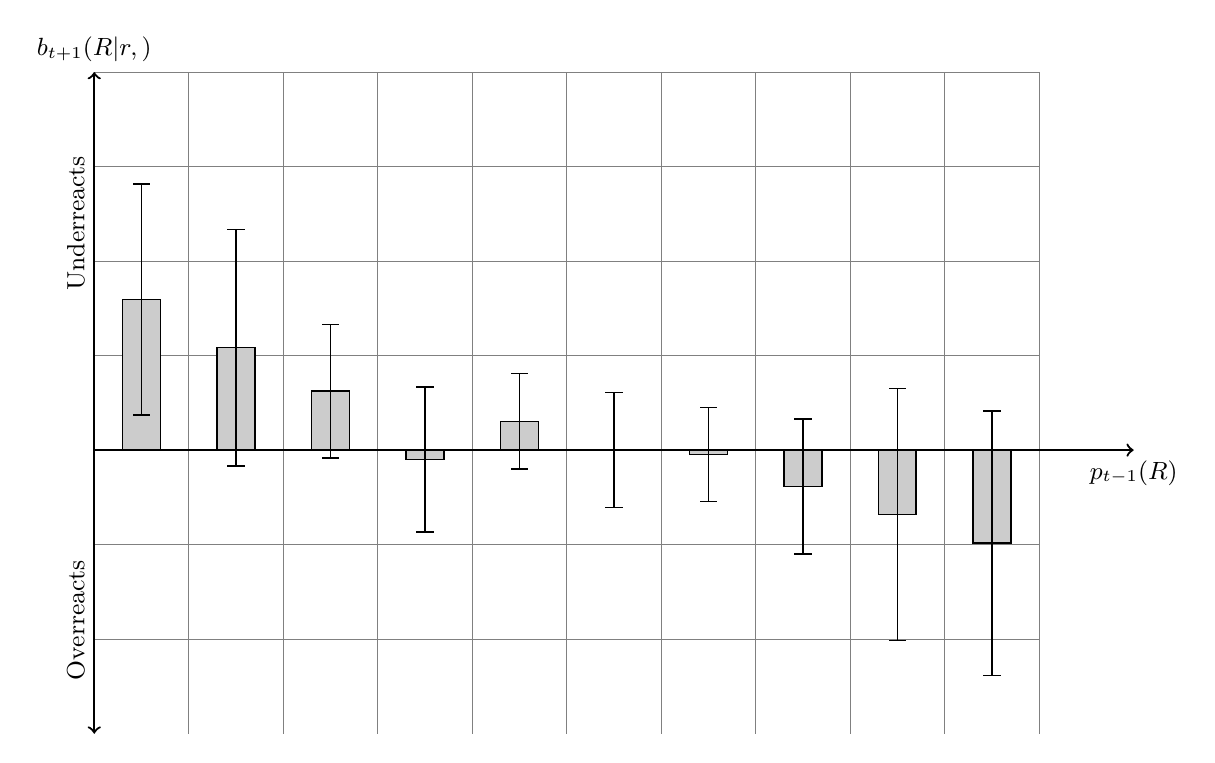
\begin{tikzpicture}[scale=12]
\draw[help lines,step=0.1] (0,-0.3) grid (1,0.4);
\filldraw[opaque,white!80!black] (0.03,0) rectangle (0.07,0.1592);
\draw[line width=0.6] (0.03,0) rectangle (0.07,0.1592);
\draw[line width=0.6,|-|] (0.05,0.0360) -- (0.05,0.2824);
\filldraw[opaque,white!80!black] (0.13,0) rectangle (0.17,0.1086);
\draw[line width=0.6] (0.13,0) rectangle (0.17,0.1086);
\draw[line width=0.6,|-|] (0.15,-0.0174) -- (0.15,0.2345);
\filldraw[opaque,white!80!black] (0.23,0) rectangle (0.27,0.0622);
\draw[line width=0.6] (0.23,0) rectangle (0.27,0.0622);
\draw[line width=0.6,|-|] (0.25,-0.0094) -- (0.25,0.1337);
\filldraw[opaque,white!80!black] (0.33,0) rectangle (0.37,-0.0100);
\draw[line width=0.6] (0.33,0) rectangle (0.37,-0.0100);
\draw[line width=0.6,|-|] (0.35,-0.0878) -- (0.35,0.0678);
\filldraw[opaque,white!80!black] (0.43,0) rectangle (0.47,0.0303);
\draw[line width=0.6] (0.43,0) rectangle (0.47,0.0303);
\draw[line width=0.6,|-|] (0.45,-0.0211) -- (0.45,0.0818);
\filldraw[opaque,white!80!black] (0.53,0) rectangle (0.57,0.0000);
\draw[line width=0.6] (0.53,0) rectangle (0.57,0.0000);
\draw[line width=0.6,|-|] (0.55,-0.0617) -- (0.55,0.0617);
\filldraw[opaque,white!80!black] (0.63,0) rectangle (0.67,-0.0046);
\draw[line width=0.6] (0.63,0) rectangle (0.67,-0.0046);
\draw[line width=0.6,|-|] (0.65,-0.0553) -- (0.65,0.0461);
\filldraw[opaque,white!80!black] (0.73,0) rectangle (0.77,-0.0387);
\draw[line width=0.6] (0.73,0) rectangle (0.77,-0.0387);
\draw[line width=0.6,|-|] (0.75,-0.1111) -- (0.75,0.0337);
\filldraw[opaque,white!80!black] (0.83,0) rectangle (0.87,-0.0682);
\draw[line width=0.6] (0.83,0) rectangle (0.87,-0.0682);
\draw[line width=0.6,|-|] (0.85,-0.2023) -- (0.85,0.0660);
\filldraw[opaque,white!80!black] (0.93,0) rectangle (0.97,-0.0986);
\draw[line width=0.6] (0.93,0) rectangle (0.97,-0.0986);
\draw[line width=0.6,|-|] (0.95,-0.2395) -- (0.95,0.0424);
\draw[line width=0.8,->]  (0,0) -- (1.1,0) node[below] {\small{$p_{t-1}(R)$}};
\draw[line width=0.8,<->] (0,-0.3) -- (0,0.4) node[above] {\small{$b_{t+1}(R|r,\xmark)$}};
\draw (0,0.24) node[above,rotate=90] {\small{Underreacts}};
\draw (0,-0.18) node[above,rotate=90] {\small{Overreacts}};
% ADD THEORY CURVE BELOW
\end{tikzpicture}
}
\subcaption{$(H_{1,1})$: 1 retraction / 1 confirmation}
\end{subfigure}
